\documentclass[titlepage]{article}
\usepackage[bottom=3cm, right=3cm, left=3cm, top=3cm]{geometry}
\usepackage {graphicx}
\usepackage{caption}
%opening
\title{%
	Practical Machine Learning\\
	
	\vspace*{2em}
	\LARGE Exercise 4\\
	Spring 2024}
\author{Lisa Stafford}
\date{March 15, 2024}

\begin{document}
	\setlength\parindent{0pt}
	
	\maketitle
	
	\section*{Abstract}
	Hyper-parameter selection is a common problem for machine learning architects where one selects the model that does the best job of generalizing and most appropriate for the given problem, but without proper knowledge of hyper-parameters within the model and what they actually do to affect the model performance, many users new to machine learning may be unaware how to select or tune hyper-parameters correctly, and most non-data scientists don't know (or may not be aware of without significant trial and error) how those hyper-parameters affect the overall runtime and performance of their model.  After selecting a base model, hyper-parameter selection remains an important part of the machine learning process.  
	
	\section*{Introduction}
	In order to learn and determine which hyper-parameters have the greatest overall effect upon the model run-time, resource use, and performance, we seek to isolate hyper-parameter selection by isolating variables in which to evaluate the performance, resource use, and runtime without changing underlying factors that may also affect model performance.  Throughout our investigation, we used a wine data set obtained from the University of Irvine \cite{dataset}. Training is performed on only the white wine within the data set.  Several models are trained implementing hyper-parameter optimization libraries directly from scikitlearn \cite{scikitlearn} and then obtaining total runtime, and training and testing performance scores and tuned hyper-parameter choices for a number of hyper-parameter tuning mechanisms.  
	

	\section*{Dataset Description}
	Our wine data set is actually comprised of two different wine subsets of data.  While both are related to variants of \cite{dataset} "Portuguese Vhinho Verde wine" the data is actually split in two subsets - one red subset and one white subset.  In this exercise, we will only be performing machine learning tasks on the white wine data set.  Each wine subset contains 11 features and 1 label for wine quality.   All features are continuous float values.  Within the model the "wine quality" labels are recognized as discrete categorical integer values ranging from 3 to 9 for the white wines.  White wine contains a total of 4898 total data instances, as shown in the following table images. Figure 1 displays feature values, statistics, and total instances for white wine.
	
	\begin{center}
	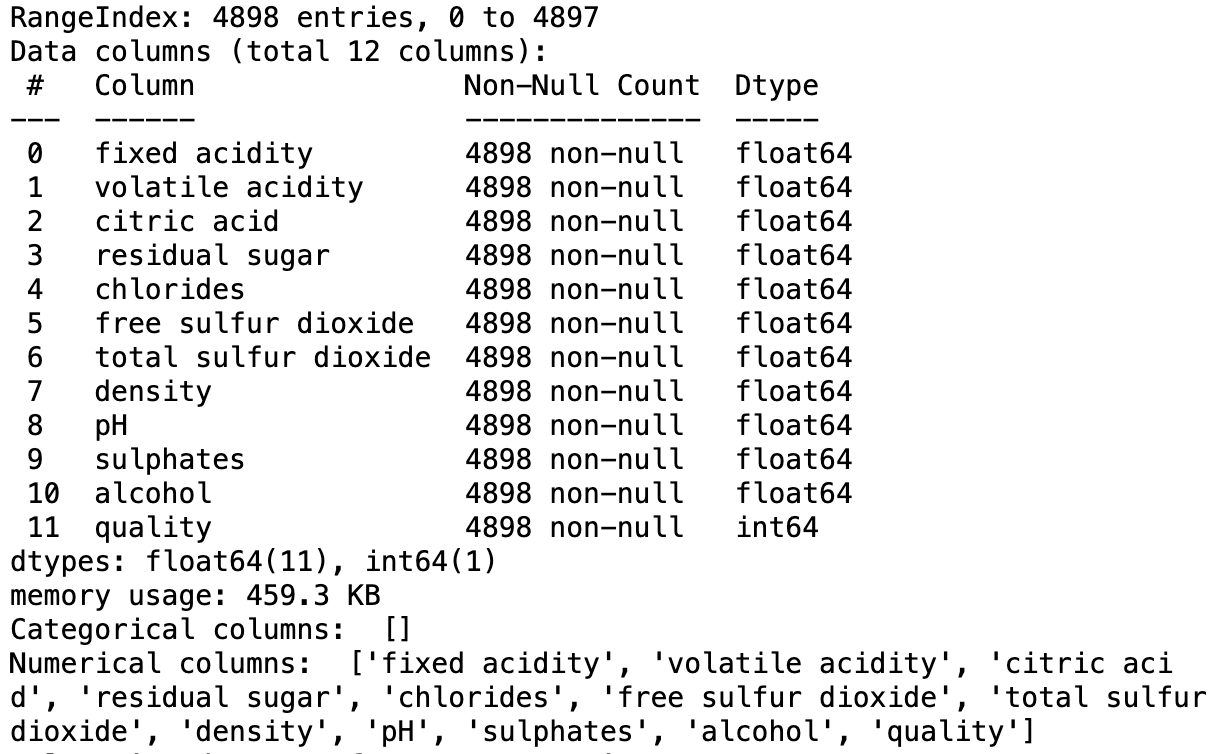
\includegraphics[width=.75\textwidth]{img/white.png}
	\end{center}

	
	\noindent As mentioned from prior exercises, white wine data is somewhat "pre-cleaned".   The feature values are all continuous and contain no missing data values.  However it should be noted that these features are not evenly distributed.  The data values are somewhat bell-shaped with a larger number of data instances with labels closer to the mean.  As described on the data set website \cite{dataset} both "data set... classes are ordered and []unbalanced] so there are many more normal wines than excellent or poor ones.... [also], both datasets have 11 physiochemical features... and a sensory output label, ('quality')".  While Standard Scaling worked best as a data transformation method in Exercise 2, we do not need to scale the data since we are only using a Random Forest Classifier as our model, and Random Forests are insensitive to data scaling.  We will however import a list of most important features obtained from an updated version of our data set exploration exercise since this does have a significant effect on the performance of Random Forest Classification models.  
	

	\section*{Experimental Setup}
		We are looking at the wine quality data set, specifically, the white wines in the data set.  From there, we're trying to predict wine quality for items within the data set to determine the best hyper-parameters and methods for finding them are done so in the most optimized way.  
		
		\vspace{.2cm}
		We know that this particular data set is supervised and the problem is a classification problem with a known number of categories. Therefore we know that the best ML models will be in that realm and since it performed consistently and very well in prior exercises, we utilize a consistent Random Forest Classifier Algorithm from scikitlearn  \cite{scikitlearn}.  Based on information from the scikitlearn website documenting use of the Random Forest Classifier library and list of selected hyper-parameters for optimization.  This list was obtained using information regarding the most valuable hyper parameters to be tuned for the Random Forest Classification Model imported from scikitlearn. 
		
		Mechanisms employed included imported scikitlearn packages including:  
	
	\begin{enumerate}
		\item Grid Search with Cross Validation ($GridSearchCV()$)
		\item Randomized Search with Cross Validation ($RandomizedSearchCV()$)
		\item Bayesian Search with Cross Validation ($BayesSearchCV()$)
	\end{enumerate}
	
	Additionally, searchers were conducted on a list of Random Forest Classifier Parameters populated from a python $dict()$ as follows:  
		 
	 \begin{enumerate} 		
	 	\item $'n\_estimators': [10, 25, 100]$
		\item $'criterion': ['gini', 'entropy', 'log\_loss']$
		\item $'max\_depth': [None, 10, 25]$
	 	\item $'bootstrap': [True, False]$
	 	\item $'warm\_start': [True, False]$
	 	\item $'n\_jobs': [-1]$
	 \end{enumerate}
	 
	\section*{Results}
	Machine learning performance results were never as highly performative as other results suggest they could be, but resulted as follows.  The highest machine learning test performance was found to be different models, depending on the wine subset.  
	\begin{center}
		 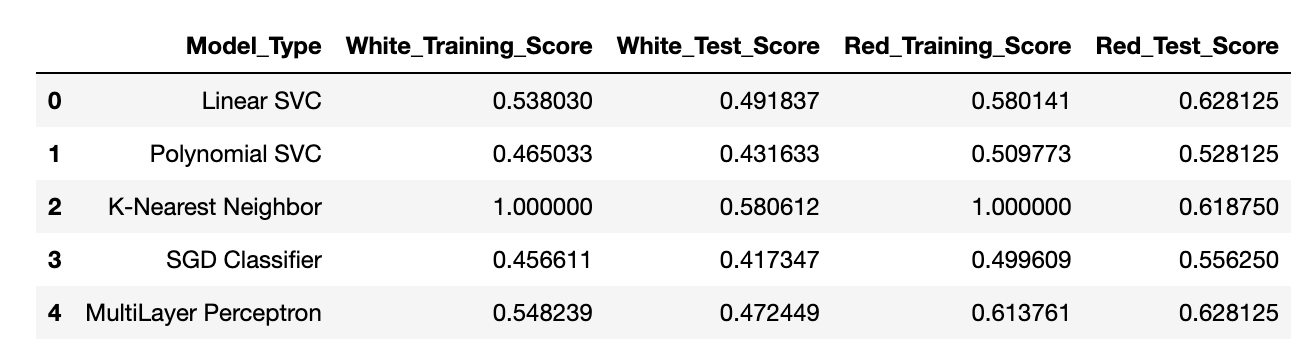
\includegraphics[width=.5\textwidth]{img/results.png}
	\end{center}
	
As shown in the chart, highest performance for the white wine subset was obtained using K-Nearest Neighbor achieving 58\% accuracy for performance on test data.  The red wine data subset resulted in the same performance for both Linear Support Vector Machine and NN using a Multi Layer Perceptron with 62.8\% accuracy for performance on test data.
	
	
\begin{thebibliography}{9}
	\bibitem{dataset} A. Asuncion, D. Newman, UCI Machine Learning Repository, University of California, Irvine  (2007).  Obtained from https://archive-beta.ics.uci.edu/dataset/186/wine+quality. 
	\bibitem{numpyisnan} C. Harris, K. Millman, S. van der Walt,  Array programming with NumPy. Nature 585, 357–362 (2020). DOI: 10.1038/s41586-020-2649-2.  https://numpy.org/doc/stable/reference/generated/numpy.isnan.html
	\bibitem{seaborn} M. Waskom, (2021). seaborn: statistical data visualization. Journal of Open Source Software, 6(60), 3021, https://doi.org/10.21105/joss.03021.
	\bibitem{scikitlearn}Scikit-learn: Machine Learning in Python, Pedregosa et al., JMLR 12, pp. 2825-2830, 2011. 
\end{thebibliography}

\end{document}
